% Aim: Develop a LaTeX script to design a simple tree diagram or hierarchical structure in the document with appropriate labels using the Tikz library. 

\documentclass[12pt, a4paper]{article}
\usepackage{tikz}

\begin{document}
	\centering
	
	\tikzstyle{level 1}=[level distance=4cm, sibling distance=6cm]
	\tikzstyle{level 2}=[level distance=4cm, sibling distance=3cm]

	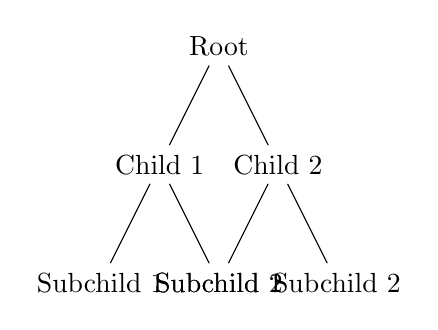
\begin{tikzpicture}[grow=down, sloped]
		
		\node {Root}
		child {
			node {Child 1}
			child {
				node {Subchild 1}				
			}
			child {
				node {Subchild 2}
			}
		}
		child {
			node {Child 2}
			child {
				node {Subchild 1} 
			}
			child {
				node {Subchild 2}
			}
		};
	\end{tikzpicture}
	
\end{document}
